\subsubsection{Data encoding (H2)}

In the base model each feature is uploaded once as an $R_Y$ rotation, so the output depends on each feature through frequencies $\{-1,0,1\}$ only. We changed the encoding while keeping the circuit, readout, loss, optimizer, and budget fixed, in three ways: (i) re-uploading, in which the feature layer is repeated before every variational layer (two uploads in the two-layer circuit and four in the four-layer circuit, with the same number of parameters); (ii) halving, and (iii) doubling the input angles. The new simulator reproduced the base VQC to within 0.0004 of test AUC, its gradients agreed with finite differences (maximum error $5\times10^{-11}$), and the output as a function of one feature contained frequencies up to 1 with one upload and up to 2 with two.

We ran these variants in two settings. First, on the four datasets with the same splits and preprocessing as before. Second, on synthetic data with controlled frequency: four features drawn uniformly in $[-\pi,\pi]$, a label given by the sign of $\sin kx_1+\sin kx_2$ (additive) or of $\sin kx_1\sin kx_2$ (product) with $k\in\{1,2,3\}$, 5\% label flips, and 600 samples, the last two features being irrelevant. Here each of the 30 seeds drew a new sample, so, unlike on the real datasets, the intervals reflect sampling of the data. All models received the same four inputs without further preprocessing, and no hyperparameter was retuned for the new settings.

\textit{With one upload, the VQC failed when the function required higher frequencies.} For $k=1$, the VQC reached a test AUC of 0.944 and 0.938 on the additive and product tasks, with gaps of 0.008 and 0.014 (Table~\ref{tab:h2synth}, Fig.~\ref{fig:h2}); its gap did not exceed that of the MLP on the additive task ($+$0.001 (95\% interval $-$0.005 to $+$0.007)) and was lower on the product task ($-$0.010 (95\% interval $-$0.018 to $-$0.001)). For $k=2$ its test AUC fell to 0.490 and 0.506, that is, to chance, while its training AUC stayed above 0.6, so the gap rose to 0.156 and 0.141, which was larger than that of the MLP ($+$0.080 (95\% interval $+$0.060 to $+$0.102) and $+$0.038 (95\% interval $+$0.016 to $+$0.062)). For $k=3$ the VQC stayed at chance (0.512 and 0.501). The failure was not exclusive to the VQC: with $k=2$ the MLP and the SVM also lost most of their performance (test AUC 0.647 and 0.632 on the additive task), whereas the Random Forest and XGBoost remained above 0.75 on the tasks with $k=2$ (0.888 and 0.785 for the Random Forest). The gap at $k=3$ was larger than at $k=1$ for the VQC, the MLP, the SVM, the Random Forest, and XGBoost on both families of tasks, whereas that of logistic regression stayed below 0.07, so the increase of the gap alone does not identify the encoding as its cause.

\begin{figure*}[t]
\centering
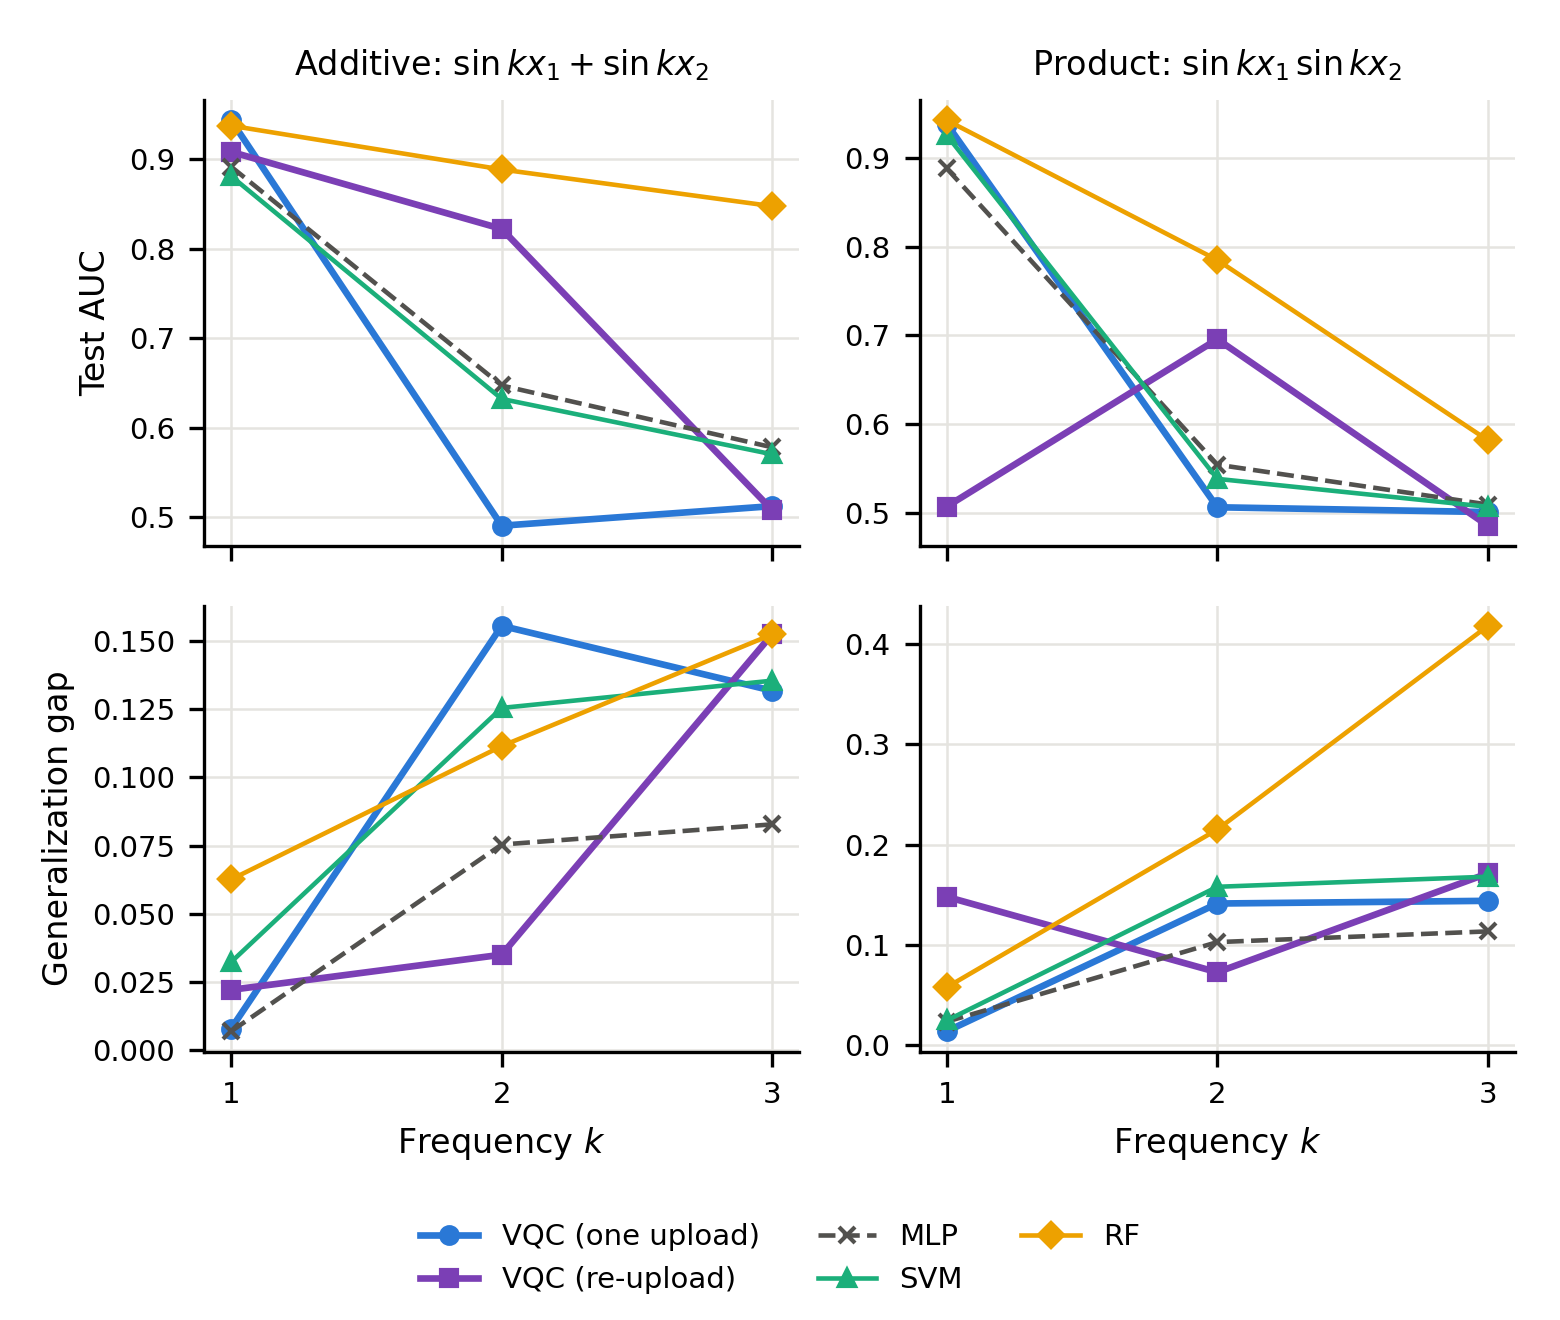
\includegraphics[width=0.62\textwidth]{fig_h2.png}
\caption{Test AUC (top) and generalization gap (bottom) as a function of the frequency $k$ of the target for the additive (left) and product (right) synthetic tasks, averaged over 30 seeds.}
\label{fig:h2}
\end{figure*}

\textit{Matching the encoding to the frequency recovered performance and reduced the gap.} For $k=2$, re-uploading raised the test AUC of the VQC by $+$0.332 (95\% interval $+$0.313 to $+$0.349) on the additive task and by $+$0.189 (95\% interval $+$0.164 to $+$0.215) on the product task, and reduced the gap ($-$0.121 and $-$0.069); with it the VQC exceeded the MLP in test AUC on both tasks ($+$0.175 and $+$0.141). Doubling the input angles, which makes the encoded frequency equal to the one of the target by construction, brought the VQC to a test AUC of 0.936 and 0.949 with gaps of 0.016 and 0.004, and, as expected, it failed for $k=1$ and $k=3$ (test AUC between 0.488 and 0.513). This shows the mechanism, not a practical remedy, because it uses knowledge of the target. For $k=3$ none of the variants learned the task (test AUC at most 0.613), although four re-uploads improved on four layers with one upload on the additive task ($+$0.111 (95\% interval $+$0.087 to $+$0.135)).

\textit{Re-uploading is not a superset of the base encoding.} With $k=1$, where the base VQC succeeded, re-uploading lowered the test AUC by $-$0.035 (95\% interval $-$0.042 to $-$0.029) on the additive task and by $-$0.431 (95\% interval $-$0.445 to $-$0.417) on the product task (to 0.507). In a probe on three seeds of the product task with $k=1$, the training AUC stayed near 0.67 and the test AUC near 0.5 with three times more epochs and with a larger initialization, so this was not a matter of optimization. The second upload follows the first variational layer, which changes the class of functions the circuit can represent, and the base circuit is not contained in it.

\begin{table*}[t]
\centering
\caption{Encoding (H2) on synthetic data with controlled frequency $k$: test AUC and generalization gap (means over 30 seeds, each with a new sample of 600 points). VQC is the base angle encoding with one upload, Re-up uploads the features before each of the two layers, and $\times$2 doubles the input angles.}
\label{tab:h2synth}
\footnotesize
\setlength{\tabcolsep}{3.5pt}
\begin{tabular}{lcccccccccccc}
\hline
 & \multicolumn{6}{c}{Test AUC} & \multicolumn{6}{c}{Gap} \\
Task & VQC & Re-up & $\times$2 & MLP & SVM & RF & VQC & Re-up & $\times$2 & MLP & SVM & RF \\
\hline
Additive, $k=1$ & 0.944 & 0.908 & 0.502 & 0.892 & 0.881 & 0.937 & 0.008 & 0.022 & 0.144 & 0.007 & 0.032 & 0.063 \\
Additive, $k=2$ & 0.490 & 0.822 & 0.936 & 0.647 & 0.632 & 0.888 & 0.156 & 0.035 & 0.016 & 0.075 & 0.126 & 0.112 \\
Additive, $k=3$ & 0.512 & 0.508 & 0.488 & 0.578 & 0.570 & 0.848 & 0.132 & 0.153 & 0.160 & 0.083 & 0.136 & 0.152 \\
\hline
Product, $k=1$ & 0.938 & 0.507 & 0.501 & 0.888 & 0.926 & 0.943 & 0.014 & 0.148 & 0.142 & 0.023 & 0.024 & 0.058 \\
Product, $k=2$ & 0.506 & 0.696 & 0.949 & 0.554 & 0.538 & 0.785 & 0.141 & 0.072 & 0.004 & 0.103 & 0.158 & 0.215 \\
Product, $k=3$ & 0.501 & 0.486 & 0.513 & 0.509 & 0.507 & 0.582 & 0.144 & 0.171 & 0.130 & 0.113 & 0.168 & 0.418 \\
\hline
\end{tabular}
\end{table*}

\textit{On the real datasets, extra frequency capacity did not help and a smaller bandwidth tended to help.} Re-uploading did not improve the test AUC on any dataset (changes of $-$0.008, $-$0.002, $-$0.002, $-$0.004 on WDBC, Ionosphere, the synthetic dataset, and Blood Transfusion; only the first interval excluded zero), and with four layers, uploading before every layer was worse than a single upload (changes of test AUC between $-$0.036 and $-$0.018 and larger gaps, by 0.017 to 0.066). Doubling the input angles lowered the test AUC on all four datasets ($-$0.083 to $-$0.029), whereas halving them left it similar or slightly higher ($+$0.004, $+$0.010, $-$0.007, $+$0.010 on WDBC, Ionosphere, the synthetic dataset, and Blood Transfusion) and reduced the gap on all four datasets ($-$0.004, $-$0.015, $-$0.011, $-$0.011, with the interval excluding zero on three of them; Table~\ref{tab:h2real}). Halving the angles also narrows their range to $[-\pi/2,\pi/2]$, which avoids mapping the two ends of each feature to the same quantum state, and we did not separate this effect from the change of bandwidth.

\begin{table*}[t]
\centering
\caption{Encoding (H2) on the four datasets: paired difference in test AUC and in generalization gap between each encoding variant and the reference indicated (mean over 30 seeds). A dagger marks a 95\% bootstrap interval that excludes zero (no multiple-comparison correction). $\times$0.5 and $\times$2 scale the input angles; Re-up uploads the features before every layer.}
\label{tab:h2real}
\footnotesize
\setlength{\tabcolsep}{4pt}
\begin{tabular}{llcccc}
\hline
Dataset & Metric & $\times$0.5 vs base & $\times$2 vs base & Re-up vs base & Re-up vs base, 4 layers \\
\hline
WDBC & $\Delta$ test AUC & $+$0.004$^{\dagger}$ & $-$0.083$^{\dagger}$ & $-$0.008$^{\dagger}$ & $-$0.018$^{\dagger}$ \\
 & $\Delta$ gap & $-$0.004$^{\dagger}$ & $+$0.022$^{\dagger}$ & $+$0.002 & $+$0.017$^{\dagger}$ \\
Ionosphere & $\Delta$ test AUC & $+$0.010 & $-$0.069$^{\dagger}$ & $-$0.002 & $-$0.036$^{\dagger}$ \\
 & $\Delta$ gap & $-$0.015 & $+$0.032$^{\dagger}$ & $-$0.001 & $+$0.050$^{\dagger}$ \\
Synthetic & $\Delta$ test AUC & $-$0.007 & $-$0.053$^{\dagger}$ & $-$0.002 & $-$0.025$^{\dagger}$ \\
 & $\Delta$ gap & $-$0.011$^{\dagger}$ & $-$0.017$^{\dagger}$ & $+$0.003 & $+$0.041$^{\dagger}$ \\
Transfusion & $\Delta$ test AUC & $+$0.010$^{\dagger}$ & $-$0.029$^{\dagger}$ & $-$0.004 & $-$0.026$^{\dagger}$ \\
 & $\Delta$ gap & $-$0.011$^{\dagger}$ & $+$0.023$^{\dagger}$ & $+$0.006 & $+$0.066$^{\dagger}$ \\
\hline
\end{tabular}
\end{table*}
